\Chapter{パズルのコーナー1.〜スリザーリンク〜(SP1)}
\Section{スリザーリンク}
\footnote{「スリザーリンク」「カックロ」の名称は(株)ニコリの登録商標です。}
\leavevmode \\
\\
\begin{figure}[h]
\centering
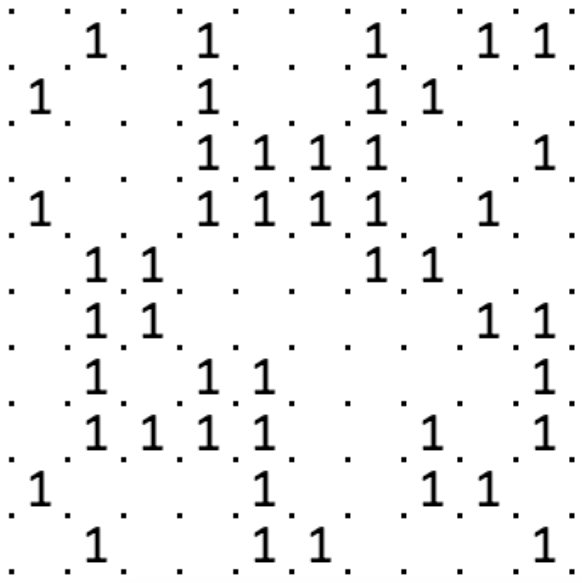
\includegraphics[width =7cm,bb = 0 0 202 202]{sp1slitherlink}
\end{figure}
\Subsection{スリザーリンクのルール}
\begin{description}
\item{1.} 点と点をタテヨコにつなげ、全体で1つの輪っかをつくります。
\item{2.}  4つの点で作られた小さな正方形の中の数字は、その正方形に引く辺の数です。数字のない小さな辺には、何本線を引くかは分かりません。
\item{3.} 線を交差させたり、枝分かれさせたりはしません。
\end{description}
